\section{Einführung}

\textbf{Definition}: \textbf{Graph} ist ein Tupel $G=(V,E)$ mit endliche Knotenmenge $V$ und endliche Kantenmenge $E$
\begin{itemize}
	\item Kante $e \in E$ hat Form $e = uv$ mit $u,v \in V$.
	\item $uv = vu$ $\rightarrow$ Graphen \textbf{ungerichtet}
	\item $e = uu$ ist erlaubt $\rightarrow$ \textbf{Schlinge}
	\item Auch $e = uv$ und $e' = uv$ erlaubt mit $e \neq e'$ $\rightarrow$ \textbf{Mehrfachkante}
	\item \textbf{Einfacher Graph} $\iff$ ohne Schlingen und Mehrfachkanten
	\item \textbf{Zusammenhängend} $\iff$ ein Weg zwischen je zwei Knoten
\end{itemize}
\bigskip
\textbf{Definition}: Eine \textbf{Zeichnung} von $G = (V,E)$ bildet diesen so auf $\R^2$ ab, dass
\begin{enumerate}
	\item Knoten Punkte in der Ebene sind, d.h. $V \subset \R^2$
	\item Kante $e = uv$ ist injektive, stetige Kurve von $u$ nach $v$, d.h. $\gamma_e\colon [0,1] \rightarrow \R^2$ mit 
	\begin{itemize}
		\item $\gamma_e(0) = u$ und $\gamma_e(1) = v$
		\item $\gamma_e(t) \notin V$ für alle $0<t<1$
	\end{itemize}
\end{enumerate}
\medskip
\begin{itemize}
	\item Zeichnung heißt \textbf{kreuzungsfrei} bzw. \textbf{planar} wenn für je zwei Kanten $e, e'$ und $0 < t, t' < 1$ gilt: $\gamma_e(t)\neq\gamma_{e'}(t')$
	\item Graph heißt \textbf{planar}, wenn er mindestens eine kreuzungsfreie Zeichnung besitzt
\end{itemize}
\bigskip
\textbf{Definition}: Für $n\in\N$ ist der \textbf{vollständige Graph} $K_n$
\begin{itemize}
	\item $V(K_n)=\{v_1,\ldots,v_n\}$
	\item $E(K_n)=\{v_iv_j\mid i,j\in \{1,\ldots,n\}, i\neq j\}$
\end{itemize}
\begin{center}
	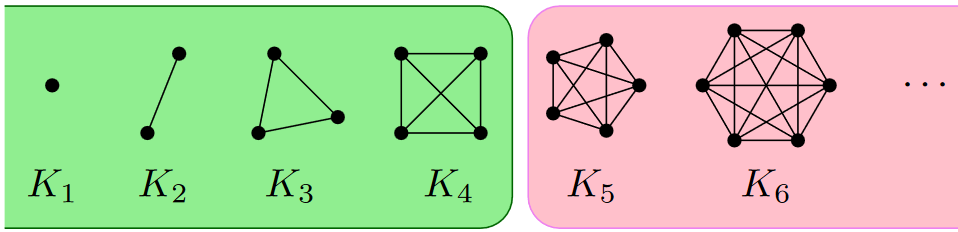
\includegraphics[width=0.6\textwidth]{images/k.png}
\end{center}

\begin{wrapfigure}{r}{0.2\textwidth}
	\centering
	\vspace{-40pt}
	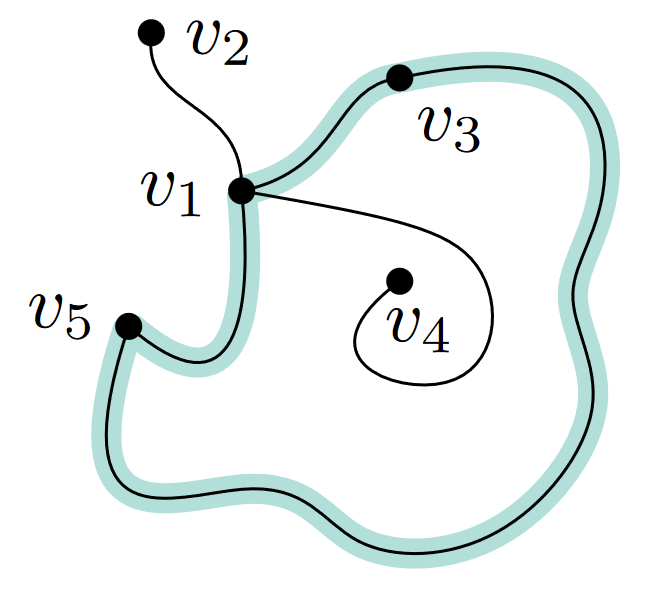
\includegraphics[width=0.2\textwidth]{images/k5-p.png}
	\vspace{40pt}
	\vspace{-120pt}
\end{wrapfigure}
\textbf{Lemma}: Graph $K_5$ ist nicht planar

\textit{Beweis}: Betrachte beliebige Zeichnung von $K_5$
\begin{itemize}
	\item Betrachte $v_1$ und seine 4 ausgehenden Kanten
	\item O.B.d.A. Kanten kreuzungsfrei zu $v_2,v_3,v_4,v_5$ in zyklischer Reihenfolge um $v_1$
	\item Kanten $v_1v_3, v_3v_5, v_5v_1$ bilden geschlossene Kurve in $\R^2$ die $v_2$ und $v_4$ trennt $\implies$ $v_2v_4$ kann nicht kreuzungsfrei gezeichnet sein
\end{itemize}
\bigskip
\textbf{Definition}: Für $m,n\in\N$ ist der \textbf{vollständig bipartite Graph} $K_{m,n}$
\begin{itemize}
	\item $V(K_{m,n})=\{a_1,\ldots,a_m\}\cup\{b_1,\ldots,b_n\}$
	\item $E(K_{m,n})=\{a_ib_j \mid i \in\{1, \ldots, m\}, j \in\{1, \ldots,n\}\}$
\end{itemize}
\begin{center}
	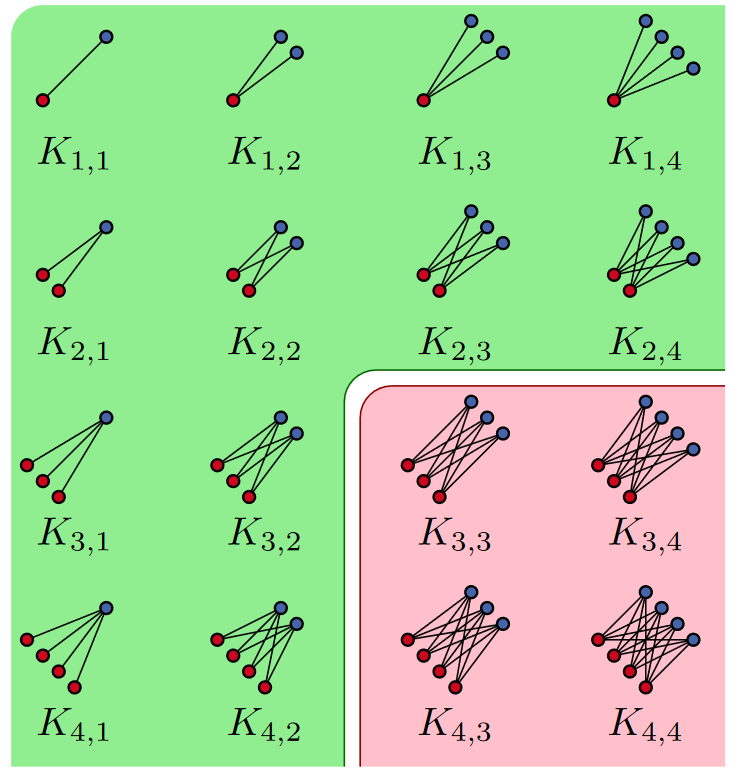
\includegraphics[width=0.4\textwidth]{images/bg.png}
\end{center}

\begin{wrapfigure}{r}{0.25\textwidth}
	\centering
	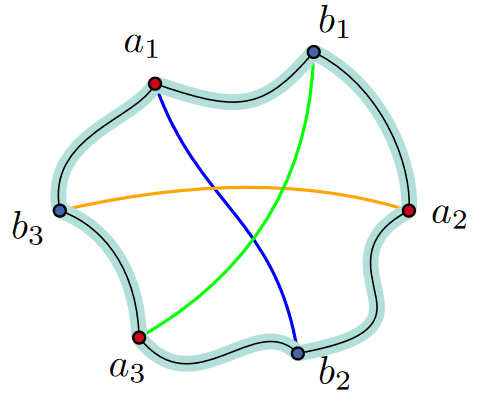
\includegraphics[width=0.25\textwidth]{images/k33-p.png}
	\vspace{-50pt}
\end{wrapfigure}
\textbf{Lemma}: Graph $K_{3,3}$ ist nicht planar

\textit{Beweis}: Betrachte beliebige Zeichnung von $K_{3,3}$
\begin{itemize}
	\item Kreis $a_1b_1a_2b_2a_3b_3$ im Graphen bildet eine geschlossene Kurve in $\R^2$
	\item Jede Kante von $a_1b_2, a_2b_3, a_3b_1$ liegt komplett innerhalb oder komplett außerhalb dieser Kurve
	
	$\implies$ mindestens zwei liegen auf der gleichen Seite
	
	$\implies$ diese zwei kreuzen sich
\end{itemize}
\bigskip
\textbf{Definitionen}: Für eine feste planare Zeichnung eines planaren Graphen definiere:
\begin{itemize}
	\item \textbf{Facetten}: Zusammenhangskomponenten von $\R^2$ nach Entfernen aller Knoten und Kanten $\implies$ Es gibt genau eine \textbf{äußere Facette} und mehrere \textbf{innere Facetten}
	\item \textbf{Äußere Knoten} sind die, die inzident zur äußeren Facette sind
	\item \textbf{Innere Knoten} sind die übrigen Knoten
	\item \textbf{Äußere Kanten} sind die, die komplett im Rand der äußeren Facette liegen 
	\item \textbf{Innere Kanten} sind die übrigen Kanten
\end{itemize}
\begin{center}
	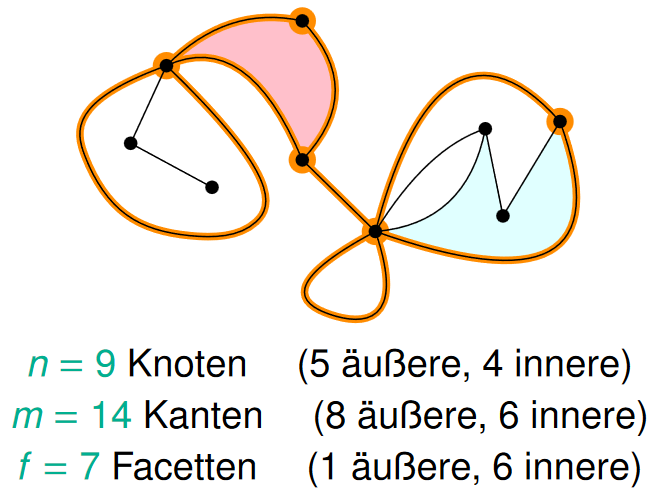
\includegraphics[width=0.4\textwidth]{images/facette.png}
\end{center}
\bigskip
\textbf{Satz von Euler}: Sei $G$ ein zusammenhängender Graph mit einer planaren Zeichnung mit $n$ Knoten, $m$ Kanten und $f$ Facetten. Dann gilt
$$n-m+f=2$$

\textit{Beweis}: Beweise $m-(f-1)=n-1$, woraus die Behauptung folgt. Führe dafür eine Induktion nach $f-1$, der Anzahl der inneren Facetten, durch.
\begin{itemize}
	\item I.A.: $f-1=0$, d.h. keine innere Facette $\rightarrow$ $G$ ist ein Baum, also kreisfrei und zusammenhängend $\rightarrow$ $m=n-1$
	\item I.S.: $f-1\geq 1$, d.h. min. eine innere Facette
	\begin{itemize}
		\item Sei $e$ eine Kante zwischen äußerer und innerer Facette $\rightarrow$ $G'=G-e$ ist zusammenhängend $\rightarrow$ In $G'$ gilt $n'=n,m'=m-1,f'=f-1$
		\item Mit I.V. folgt: $m'-(f'-1)=n'-1\Leftrightarrow m-1-(f-1-1)=n-1 \Leftrightarrow m-(f-1)=n-1$
	\end{itemize}
\end{itemize}
\begin{center}
	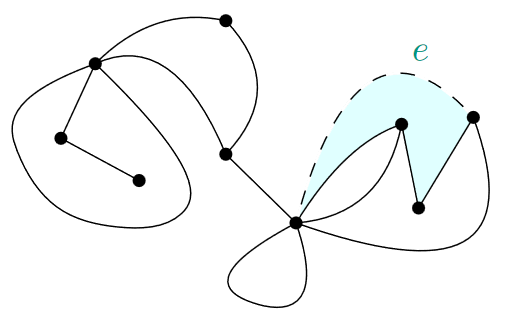
\includegraphics[width=0.3\textwidth]{images/euler-proof.png}
\end{center}
\bigskip
\textbf{Korollar aus Euler-Formel}: Sei $G$ ein planarer, einfacher Graph mit $n\geq 3$ Knoten, $m$ Kanten, und kleinstem vorkommenden Knotengrad $\delta(G)$.
Dann gilt 
$$m\leq 3n-6\qquad\text{ und }\qquad \delta(G)\leq 5$$

Beide Ungleichungen sind bestmöglich.

\pagebreak
\textit{Beweis}: $m\leq 3n-6$
\begin{itemize}
	\item O.B.d.A. $G$ ist zusammenhängend, da man Kanten einfügen kann bis er das ist
	\item Jede Facette ist berandet von min. 3 Kantenseiten, da $n\geq 3$ 
	\item Jede Kantenseite in genau 1 Facette
	\item Jede Kante hat genau 2 Seiten
\end{itemize}
$\implies 3f\leq \text{Anzahl der Seiten-Facetten-Inzidenzen} =2m$

$\implies 3(2+m-n)\leq 2m \implies m\leq 3n-6$ (mit Euler-Formel)\\

\textit{Beweis}: $\delta(G)\leq 5$
\begin{itemize}
	\item Jede Kante hat genau 2 inzidente Knoten
	\item Jeder Knoten $v$ hat genau $\text{deg}(v)$ inzidente Kanten
	\item Für jeden Knoten $v$ gilt $\text{deg}(v)\geq\delta(G)$
\end{itemize}
$\implies 2m=\text{Anzahl der Knoten-Kanten-Inzidenzen}=\sum\limits_{v\in V(G)}\text{deg}(v)\geq \delta(G)\cdot n$

$\implies 2(3n-6)\geq 2m\geq \delta(G)\cdot n \implies \delta(G)\leq 6-12/n$

